\documentclass{article}
\usepackage{acro}
\usepackage[backend=biber,style=vancouver]{biblatex}
\usepackage[inline]{enumitem}
\usepackage{amsmath}
\usepackage{cleveref}
\usepackage{pgfplots}
\usepackage{import}
\usepackage{booktabs}
\usepackage{makecell}
\usepackage{todonotes}
\usepackage{xcolor}
\usepackage{subcaption}
\usepackage{pgfplots}
\usepackage{pgfplotstable}
\usepackage{tabularx}
\usepackage{authblk}

\usepackage[margin=1in]{geometry}

\usepgfplotslibrary{groupplots}
\usepgfplotslibrary{colorbrewer}

% Custom commands
\definecolor{gdvGreen}{HTML}{00B000}
\definecolor{gdvOrange}{HTML}{FFAA00}
\definecolor{gdvRed}{HTML}{E9002D}

\newcommand{\skill}{{\color{gdvGreen}{$\pmb{+}$}}}
\newcommand{\noskill}{{\color{gdvOrange}{$\pmb{-}$}}}
\newcommand{\snoskill}{{\color{gdvRed}{$\pmb{/}$}}}

% Layout
\usepackage[font=small]{caption}
\renewcommand\Affilfont{\small}

\pgfplotsset{every tick label/.append style={font=\footnotesize}}
\pgfplotsset{every axis label/.append style={font=\footnotesize}}
\pgfplotsset{every axis legend/.append style={font=\footnotesize}}

\renewcommand*{\bibfont}{\footnotesize}

\renewcommand{\maketitle}{
	\begin{flushleft}
		{\LARGE \@title \par}
		\vskip 1em
		\@author
		\vskip 1em
			{\large \@date \par}
	\end{flushleft}
}
\makeatletter

% Left-align abstract heading and content
\renewenvironment{abstract}{\section*{Abstract}}{}


% Draft
\usepackage{setspace}
\doublespacing%
\usepackage{lineno}
\linenumbers%

% Preamble
% Declared acronyms
\DeclareAcronym{aac}{
  short=AAC,
  long=assistive and augmentative communication
}
\DeclareAcronym{bci}{
  short=BCI,
  long=brain-computer interface,
}
\DeclareAcronym{eeg}{
  short=EEG,
  long=elec\-tro\-en\-ce\-pha\-lo\-gra\-phy
}
\DeclareAcronym{ecog}{
  short=ECoG,
  long=elec\-tro\-cor\-ti\-co\-gra\-phy
}
\DeclareAcronym{erp}{
  short=ERP,
  long=event-related potential
}
\DeclareAcronym{als}{
  short=ALS,
  long=Amyotrophic Lateral Sclerosis
}
\DeclareAcronym{ms}{
  short=MS,
  long=Multiple Sclerosis
}
\DeclareAcronym{sma}{
  short=SMA,
  long=Spinal Muscular Atrophy
}
\DeclareAcronym{dmd}{
  short=DMD,
  long=Duchenne's Muscular Dystrophy
}
\DeclareAcronym{lis}{
  short=LiS,
  long=Locked-in Syndrome
}
\DeclareAcronym{vsa}{
  short=VSA,
  long=visuospatial attention
}
\DeclareAcronym{itr}{
  short=ITR,
  long=information transfer rate
}
\DeclareAcronym{ssvep}{
  short=SSVEP,
  long=steady-state visually evoked potential
}
\DeclareAcronym{cvep}{
  short=cVEP,
  long=code-modulated visually evoked potential
}
\DeclareAcronym{mvep}{
  short=mVEP,
  long=motion-onset visually evoked potential
}
\DeclareAcronym{vep}{
  short=VEP,
  long=visually evoked potential
}
\DeclareAcronym{csp}{
  short=CSP,
  long=common spatial patterns
}
\DeclareAcronym{cca}{
  short=CCA,
  long=canonical correlation analysis
}
\DeclareAcronym{lda}{
  short=LDA,
  long=linear discriminant analysis
}
\DeclareAcronym{rocauc}{
  short=ROC-AUC,
  long=area under the receiver-operator characteristic curve
}
\DeclareAcronym{snr}{
  short=SNR,
  long=signal-to-noise ratio
}
\DeclareAcronym{ica}{
  short=ICA,
  long=independent component analysis
}
\DeclareAcronym{pca}{
  short=PCA,
  long=principal component analysis
}
\DeclareAcronym{cble}{
  short=CBLE,
  long=Classifier-based Latency Estimation
}
\DeclareAcronym{wcble}{
  short=WCBLE,
  long=Classifier-based Latency Estimation with Woo\-dy iterations
}
\DeclareAcronym{tlda}{
  short=tLDA,
  long=block-Toeplitz linear discriminant analysis
}
\DeclareAcronym{lcmv}{
  short=LCMV,
  long=linearily constrained minimum-variance
}
\DeclareAcronym{isi}{
  short=ISI,
  long=inter-stimulus interval
}
\DeclareAcronym{tbi}{
  short=TBI,
  long=traumatic brain injury
}
\DeclareAcronym{fa}{
  short=FRDA,
  long=Friedreich's Ataxia
}
\DeclareAcronym{sspi}{
  short=SSPI,
  long=severe speech and physical impairment
}
\DeclareAcronym{sspgi}{
  short=SSPGI,
  long={severe speech, physical and gaze impairment}
}
\DeclareAcronym{eog}{
  short=EOG,
  long=electrooculogram
}
\DeclareAcronym{rsvp}{
  short=RSVP,
  long=rapid serial visual presentation
}
\DeclareAcronym{hoda}{
  short=HODA,
  long=Higher Order Discriminant Analysis
}
\DeclareAcronym{bttda}{
  short=BTTDA,
  long=Block-Term Tensor Discriminant Analysis
}
\DeclareAcronym{cp}{
  short=CP,
  long=cerebral palsy
}
\DeclareAcronym{mi}{
  short=MI,
  long=motor imagery
}
\DeclareAcronym{stbf}{
  short=STBF,
  long=spatiotemporal beamformer
}
\DeclareAcronym{stbf-struct}{
  short=STBF-struct,
  long=structured spatiotemporal beamformer
}
\DeclareAcronym{stbf-emp}{
  short=STBF-emp,
  long=STBF with empirical covariance
  estimation
}
\DeclareAcronym{stbf-shrunk}{
  short=STBF-shrunk,
  long=STBF with shrunk covariance estimation
}
\DeclareAcronym{loocv}{
	short=LOOCV,
	long=leave-one-out cross-validation
}
\DeclareAcronym{svm}{
	short=SVM,
	long=support vector machine
}
\DeclareAcronym{hosvd}{
	short=HOSVD,
	long=Higher Order Singular Value Decomposition
}
\DeclareAcronym{ucd}{
	short=UCD,
	long=user-centered design,
}

\addbibresource{references.bib}

\author[1,2,*]{Arne Van Den Kerchove}
\author[2]{Juliette Meunier}
\author[3]{Marie de Moura}
\author[4]{Alixe Willemssens}
\author[5]{Dorien Geurinckx}
\author[4]{Edward Schiettecatte}
\author[6]{Philip Van Damme}
\author[2]{Hakim Si-Mohammed}
\author[2]{François Cabestaing}
\author[7]{Etienne Allart}
\author[1]{Marc M. Van Hulle}

\affil[1]{%
	Leuven Brain Institute;
	Leuven.AI;
	KU Leuven,
	Department of Neurosciences,
	Laboratory for Neuro- and Psychophysiology,
	Campus Gasthuisberg,
	Herestraat 49 bus 1021,
	BE-3000 Leuven,
	Belgium
}
\affil[2]{%
	Univ. Lille, CNRS, Centrale Lille,
	UMR 9189 CRIStAL,
	Bâtiment ESPRIT,
	Avenue Henri Poincaré,
	F-59655 Villeneuve d'Ascq,
	France
}
\affil[3]{%
	Fondation Partage et Vie,
	24 Rue des Fleurs,
	F-59120 Loos,
	France
}
\affil[4]{%
	TRAINM Neuro Rehab Clinics,
	Quellinstraat 38,
	BE-2018 Antwerp,
	Belgium
}
\affil[5]{%
	KU Leuven,
	Department of Neurosciences,
	Laboratory for Experimental Neurology;
	VIB,
	Laboratory of Neurobiology,
	Center for Brain and Disease Research;
	University Hospitals Leuven
	Department of Neurology,
	Campus Gasthuisberg,
	Herestraat 49,
	BE-3000 Leuven,
	Belgium
}
\affil[6]{%
	University Hospitals Leuven
	Department of Neurology,
	Campus Gasthuisberg,
	Herestraat 49,
	BE-3000 Leuven,
	Belgium
}
\affil[7]{%
	CHU de Lille,
	Service de Rééducation Neurologique Cérébrolésion,
	Univ. Lille, UFR3S médecine,
	Lille Neuroscience and Cognition,
	Hôpital Swynghedauw,
	Rue André Verhaeghe,
	F-59000 Lille
}
\affil[*]{Corresponding author, \texttt{arne.vandenkerchove@kuleuven.be}}

\title{%
	Visual ERP-based brain-computer interface use with with severe speech,
	physical, speech and eye movement impairments: case studies
}

\begin{document}

\maketitle
\todo{Please double check your contact and authorship information}

\begin{abstract}
	\noindent
	\emph{Background:}
	Individuals with severe speech and physical impairment face significant challenges in
	communication and	daily interaction.
	Visual \acp{bci} offer a potential assistive solution, but their usability is
	limited when facing eye motor impairments that affect gaze fixation
	and \ac{vsa}.
	This study investigates the feasibility of a gaze-independent visual oddball
	\ac{bci} for individuals with severe eye motor impairment in addition to
	physical and speech impairment.
	\emph{Methods:}
	Seven participants with varying degrees of eye motor impairments were
	recruited and \ac{bci} decoding accuracy evaluated under three conditions:
	overt, covert, and free \ac{vsa} using multiple classification methods.
	\emph{Results:} covert \ac{vsa} with central fixation leads to decreased
	accuracy, whereas uncued \ac{vsa} is comparable to overt \ac{vsa} in some
	gaze-impaired participants.
	Furthermore, cross-condition decoder training and evaluation suggests that training
	with overt \ac{vsa} may improve performance in gaze-impaired individuals.
	\emph{Conclusions:}
	These findings highlight the need for adaptive decoding strategies and further
	validation in applied settings used by impaired individuals.
\end{abstract}

\noindent
\paragraph{Keywords:}
brain-computer interface,
assistive and augmented communication
event-related potential,
covert visuospatial attention,
eye motor impairment,
decoding

\acresetall%
\section{Background}
Neurological conditions, such as acquired brain lesions,
neuromuscular disorders and \ac{als} can result in severe speech and physical impairment.
This, in turn, significantly alters an individual's ability to communicate and interact
with their environment, reducing the level of activity and participation,
and overall quality of life.
\Ac{aac} technology~\cite{Ascari2018,Elsahar2019,Curtis2022} leveraging visual \acp{bci}\cite{Schultz2017, Peters2022},
which relies on the interpretation of visual stimuli by the user,
offers several advantages in this context.
The rapid stimulation pace of visual \acp{bci} and the modulation of
information over spatial attention allow for high \acp{itr}~\cite{Abiri2019,Han2023}.
Combined with their ability to operate with non-invasive recording technology,
this makes them well-suited for real-time communication tasks.

However, severe visual impairments such as nystagmus (uncontrolled eye movements), diplopia (double
vision), ophthalmoplegia (eye paralysis) fatigability and head motion
limitations can significantly hinder the ability to use visual BCIs.
These impairments make it difficult for
\ac{bci} users to track or focus on visual stimuli accurately, reducing their
performance with BCIs that rely on visual cues~\cite{McCane2014,FriedOken2020,Pasqualotto2015}.
Unfortunately, it is again for this group that eye tracking solutions also
perform poorly, making them more reliant on potential developments in \acp{bci}
that do not rely on eye gaze.

Eye motor impairments are presumed to reduce performance in operating visual
\acp{bci}~\cite{VanDenKerchove2024a}, since users
cannot comfortably redirect their gaze at the desired target,
i.e., perform overt \ac{vsa}.
This is usually circumvented by designing gaze-independent \acp{bci}~\cite{Riccio2012}.
These interfaces either avoid visual stimulation or exploit some form of
covert \ac{vsa}, where gaze and \ac{vsa} do not coincide.

Several studies on visual oddball \acp{bci} indicate that performance declines
without fixation on the intended target~\cite{Brunner2010, Treder2010, RonAngevin2019},
necessitating gaze-independent solutions.
These studies build on the assumption that \ac{bci} users with eye motor
impairment would feel comfortable operating an interface in pure covert \ac{vsa} with
central fixation.
One could argue that a \ac{bci} verified to work only with central fixation could
also be considered gaze-dependent.
This does not account for the residual eye motor capabilities of most individuals
with \ac{sspgi}, the (dis)comfort they experience while performing gaze fixation
and other confounding factors resulting from their eye
motility.

It is notable that studies reporting on
gaze-independent visual \ac{bci} use by individuals with \ac{sspgi} are very few.
Results are usually different from those obtained with healthy control
participants, due to difference in capabilities, brain
response, equipment and environment.

\textcite{Lesenfants2014} tested a \ac{bci} using gaze-independent \acp{ssvep} in six
participants with \ac{lis} yet they only exceeded chance level accuracy in two.
More recently, \textcite{Peters2020} performed a trial with two
participants with late-stage \ac{als} with severe visual impairment.
Their \ac{ssvep} paradigm was not optimized for gaze-independence, but the
system showed high accuracy, outperforming an eye tracking alternative.
It would be of interest to determine whether such results can be replicated with
participants with other neurological conditions, and with a visual oddball rather
than an \ac{ssvep} paradigm.

\textcite{Orhan2012} and \textcite{Oken2014} tested the \ac{rsvp} speller with
individuals with \ac{lis}. Due to the serial nature of the stimulation paradigm,
communication was rather slow but they demonstrated viability of the \ac{rsvp}
paradigm in a relevant target population.

\textcite{Severens2014} evaluated the visual Hex-o-Spell~\cite{Treder2010} on 5
participants with \ac{als} and showed that this visual oddball interface optimized
for gaze-independence can outperform a tactile \ac{bci}.
While this speaks to the power of visual paradigms even in groups that are
expected to have eye motor impairment, they did not verify the gaze direction
of participants during the experiment.
It was assumed that participants were performing overtly.
Participants with \ac{als} also exhibited a substantially lower accuracy than healthy
controls (58\% vs. 88\%).

\textcite{VanDenKerchove2024} also built towards a gaze-independent solution
using the visual Hex-o-Spell interface~\cite{VanDenKerchove2024}.
They partially accounted for the fact that \ac{bci} users with \ac{sspgi} might
not fully rely on central gaze fixation by evaluating settings independent of
central fixation.
They showed gaze-independent performance can be improved in healthy subjects by
using a suited decoding strategy that corrects for latency jitter in covert \ac{vsa} responses.
Yet, there is a need for verification of these results in individuals with
\ac{sspgi}.

Ultimately, this research aims to develop gaze-independent \ac{bci} for
individuals who are fully locked-in and have no alternative means of communication.
However, this group is very small and it is often challenging to recruit them
into a study and perform experiments~\cite{Wolpaw2006}.
Individuals with less severe paralysis or in less progressed disease stages that struggle with
eye-tracking technology could also benefit from
solutions tailored to their specific situation and remaining capabilities.
Therefore, we apply the concepts from earlier work and literature to
individuals with severe speech and physical impairment affected by various degrees of eye motor impairment
using a visual oddball \ac{bci}.
The contributions of this study are as follows:
\begin{enumerate*}[label={(\arabic*)}]
	\item recruit individuals that are specifically affected with \ac{sspgi} in
	      a visual \ac{bci} study.
	\item explore their capabilities and experienced comfort when operating such a \ac{bci},
	\item evaluate the performance of a gaze-independent visual \ac{bci} for this
	      group,
	\item verify if this performance can be improved with a suitable decoding
	      strategy.
\end{enumerate*}
Finally, we formulate a set of recommendations based on our experience with carrying out this study
that could be leveraged for the design of further similar studies or \ac{bci}-\ac{aac} solutions for this target population.


\section{Methods}
\subsection{Recruitment}
Participants were recruited from the Neuromuscular Reference center at
University Hospital Leuven (Leuven, Belgium), TRAINM Neuro Rehab Clinics
(Antwerp, Belgium), the Neurorehabilitation Unit at the Lille University
Medical Center (Lille, France), and Fondation Partage et Vie (Loos,
France).
Experiments were performed under the supervision of the treating physician.

In order to be recruited, participants must:
\begin{enumerate}
	\item be at least 18 years old and no older than 60
	      years,
	\item belong to class 2 or 3 according to the \ac{bci}	user selection criteria
	      presented by~\textcite{Wolpaw2006},%
	      \label{item:patients/inclusion/wolpaw}
	\item have limitations to the extent or comfort of their eye motor control
	      (partial or full gaze paralysis, uncontrolled gaze movements, or conditions affecting the capability to direct the gaze or fixate.)%
	      \label{item:patients/inclusion/oculomotor}
	\item have given their informed consent prior to participation.
\end{enumerate}
Participants were excluded if they:
\begin{enumerate}
	\item had a diagnosis of a major medical condition, including any major
	      neurological or psychiatric disorder other than those of interest based on
	      inclusion criteria~\ref{item:patients/inclusion/wolpaw},
	      and~\ref{item:patients/inclusion/oculomotor}\label{item:patients/exclusion/medical}
	\item had a predisposition to or a history of any kind of epileptic seizures,
	      including photosensitive epilepsy,\label{item:patients/exclusion/epilepsy}
	\item had a severe loss in vision or hearing that would significantly impair
	      participation in the experiment,\label{item:patients/exclusion/vision}
	\item were using specific psychoactive medications or substances that could affect the outcome.
	      (neuroleptics or benzodiazepines)%
	      \label{item:patients/exclusion/cognitive}
	\item were unable to understand the experiment instructions and cooperate,
	\item had any other limitations preventing them from performing the given task.
\end{enumerate}

In total, 11 individuals were contacted. Of these, one person with
\ac{ms} was excluded based on criterion~\ref{item:patients/exclusion/vision}.
One person recovering from \ac{tbi} was excluded based on both~\ref{item:patients/exclusion/epilepsy}
and~\ref{item:patients/exclusion/cognitive}, and one person recovering from
stroke based on~\ref{item:patients/exclusion/medical}.
One further person recovering from a stroke was excluded due to technical
difficulties during the experimental session.

Ultimately, 7 participants were retained.
Of these, one participant was diagnosed with bulbar-onset \ac{als}, three with
\ac{fa} an three were recovering from \ac{lis} due to stroke.
Table~\ref{tab:patients/patients} lists the included participants and their
diagnoses, each case is clinically described in \cref{app:clinical-eval}.
\begin{table*}
	\footnotesize
	\footnotesize
\begin{tabularx}{\linewidth}{@{}Xlrrrlllrr@{}}
	\toprule
	\textbf{ID}     & \textbf{Diagnosis}            & \textbf{Age}           & \textbf{Sex} & \textbf{Hand.} &
	\textbf{Speech} & \textbf{Trach.}               & \textbf{Communication} &
	\textbf{W}      & \textbf{KB}                                                                                                                      \\ \midrule
	PA1             & bulbar-onset \acs{als}        & 58                     & M            & L              & anarthric  & no  & tablet       & 3 & 4 \\
	PB1             & \acs{fa}                      & 41                     & M            & L              & dysarthric & no  & verbal       & 3 & 3 \\
	PB2             & \acs{fa}                      & 43                     & F            & R              & dysarthric & no  & verbal       & 3 & 3 \\
	PB4             & \acs{fa}                      & 48                     & M            & R              & dysarthric & no  & verbal       & 3 & 3 \\
	PC2             & ischemic brainstem stroke     & 43                     & M            & R              & anarthric  & yes & eye movement & 2 & 4 \\
	PC3             & haemorrhagic brainstem stroke & 43                     & F            & R              & anarthric  & yes & letterboard  & 2 & 3 \\
	PC4             & ischemic brainstem stroke     & 54                     & M            & R              & anarthric  & yes & letterboard  & 2 & 3 \\
	\bottomrule
\end{tabularx}

	\caption{Included participants with their diagnosis and relevant communication
		capabilities.
		W:\ classification according
		to~\textcite{Wolpaw2006}, KB:\ classification according
		to~\textcite{Kuebler2008}.
	}%
	\label{tab:patients/patients}
\end{table*}


\subsection{Visual skill and eye motor examination}

Self-reported eye motor and visual abnormalities or those observed in clinical
assessment are reported in~\cref{tab:patients/eye}
Visual skills were assessed using the framework established by \textcite{FriedOken2020}.
These describe on a higher level the factors that can reduce visual \ac{bci} performance when impaired,
and include visual acuity, visual fixation, eyelid function, ocular motility,
binocular vision, and field of vision.
Additionally, participants and their caregivers were asked about eye tremors
(nystagmus or other) and other involuntary eye movements.
Vision was assessed using a logMAR chart~\cite{Bailey1976}.
%As an objective metric, we implemented and performed the automated NeuroEye eye movement
%test proposed by~\textcite{Hassan2022} using calibration-free eye tracking to
%check if it revealed any further eye motor abnormalities.
%This was not the case.
\begin{table*}
	\begin{tabular}{@{}lccccccc@{}}
	\toprule
	                     & PA1      & PB1      & PB2       & PB4      & PC2       & PC3       & PC4       \\
	\midrule
	Visual fixation      & \noskill & \noskill & \noskill  & \noskill & \noskill  & \noskill  & \noskill  \\
	Eyelid function      & \skill   & \skill   & \skill    & \skill   & \skill    & \noskill  & \noskill  \\
	Ocular motility      & \skill   & \noskill & \skill    & \noskill & \snoskill & \snoskill & \noskill  \\
	Binocular vision     & \skill   & \skill   & \skill    & \skill   & \noskill  & \snoskill & \snoskill \\
	Field of vision      & \skill   & \skill   & \skill    & \skill   & \skill    & \snoskill & \noskill  \\
	Involuntary movement & \skill   & \noskill & \snoskill & \noskill & \noskill  & \noskill  & \skill    \\
	\midrule
	Visual acuity        & 0.0      & 0.0      & 0.6       & 0.2      & 0.0       & 0.0       & 0.6       \\
	\bottomrule
\end{tabular}

	\caption[Visual skills of the included participants.]{%
		Self-reported visual skills as defined by \textcite{FriedOken2020} of
		gaze-impaired participants included in this study.
		\skill\ skilled, \noskill\ impaired, \snoskill\ severely impaired.
		Visual acuity was assessed using the logMAR scale (lower is better).
	}%
	\label{tab:patients/eye}
\end{table*}

All participants reported some degree of fatigue or discomfort when fixating.
Participant PA1 had the mildest impairment, only reporting fatigue when fixating
for prolonged times.
The \ac{fa} participants were mostly affected by eye tremors and impaired pursuit.
Eye motor function of participants PC2, PC3, and PC4, those recovering from
brain stem and cerebellar stroke, was most severely affected.



Finally, we also recorded gaze position throughout the experimental session to
register the participant's gaze relative to the stimulated \ac{bci} targets,
using a Tobii X2-30 Compact (Tobii Technology AB, Sweden) portable eye tracker placed at the bottom of the laptop screen.
The registered data was cleaned by fusing left and right eye screen-based gaze
coordinates into one channel for the horizontal and one for vertical gaze position.
If both were present for a given sample, the fused channel was the mean of both
values.
If at a given sample either the left or the right eye was not detected for a
given channel, the value of the other one was adopted.
If both were missing, the gaze position remained unset at that time point, and no
interpolation was performed.



\subsection{\Acs{bci} stimulation}

The \ac{bci} stimulation procedure was based on the
Hex-o-Spell~\cite{Treder2010} implementation presented
by~\textcite{VanDenKerchove2024}.
Similar to this study, the task consists of counting the flashes of a cued
target among 6 circular, flashing targets laid out in a hexagonal pattern in the
field of view of the user as displayed
in~\cref{fig:methods/stimulation/stimulation}.
We refer to \textcite{VanDenKerchove2024} for further details on the implementation
of the stimulation procedure.
\begin{figure*}
	\centering
	\begin{subfigure}[b]{.41\textwidth}
		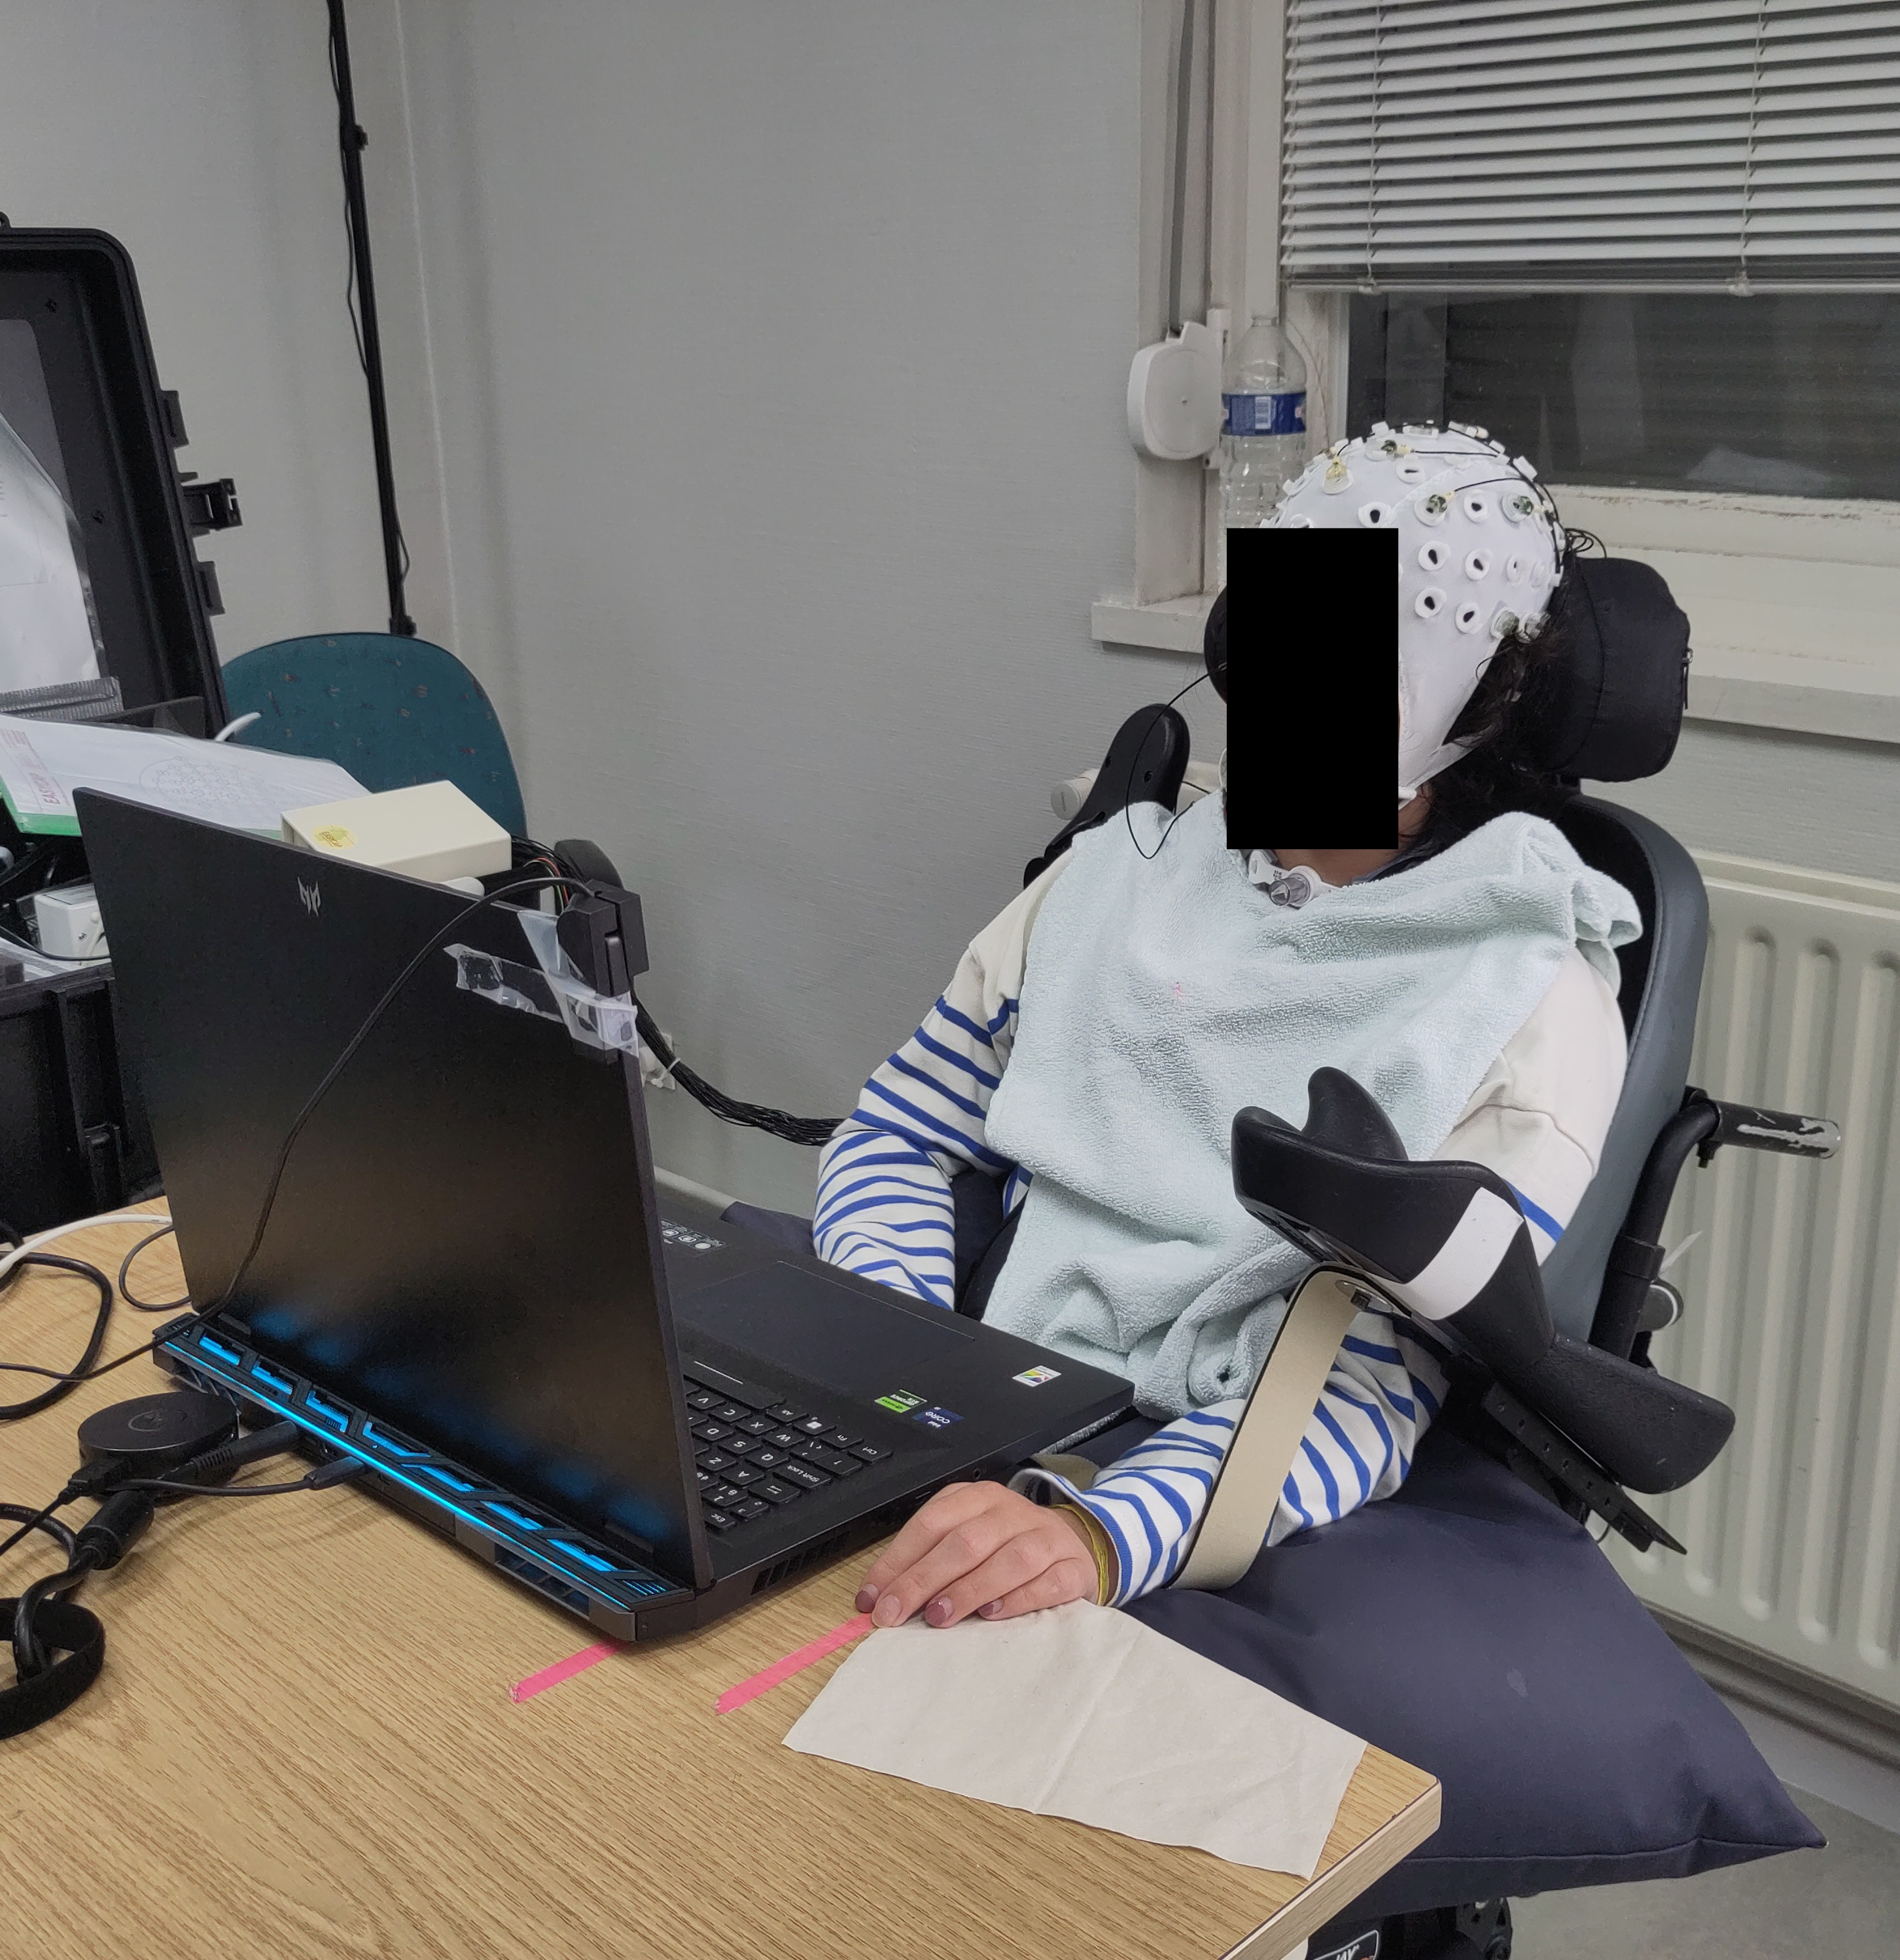
\includegraphics[width=\textwidth]{figures/PD01b-obfuscated.jpg}
		\caption{A participant seated in a wheelchair in front of the stimulation laptop with EEG
			cap.}
	\end{subfigure}\hfill%
	\begin{minipage}[b]{.54\textwidth}
		\begin{subfigure}[b]{.45\linewidth}
			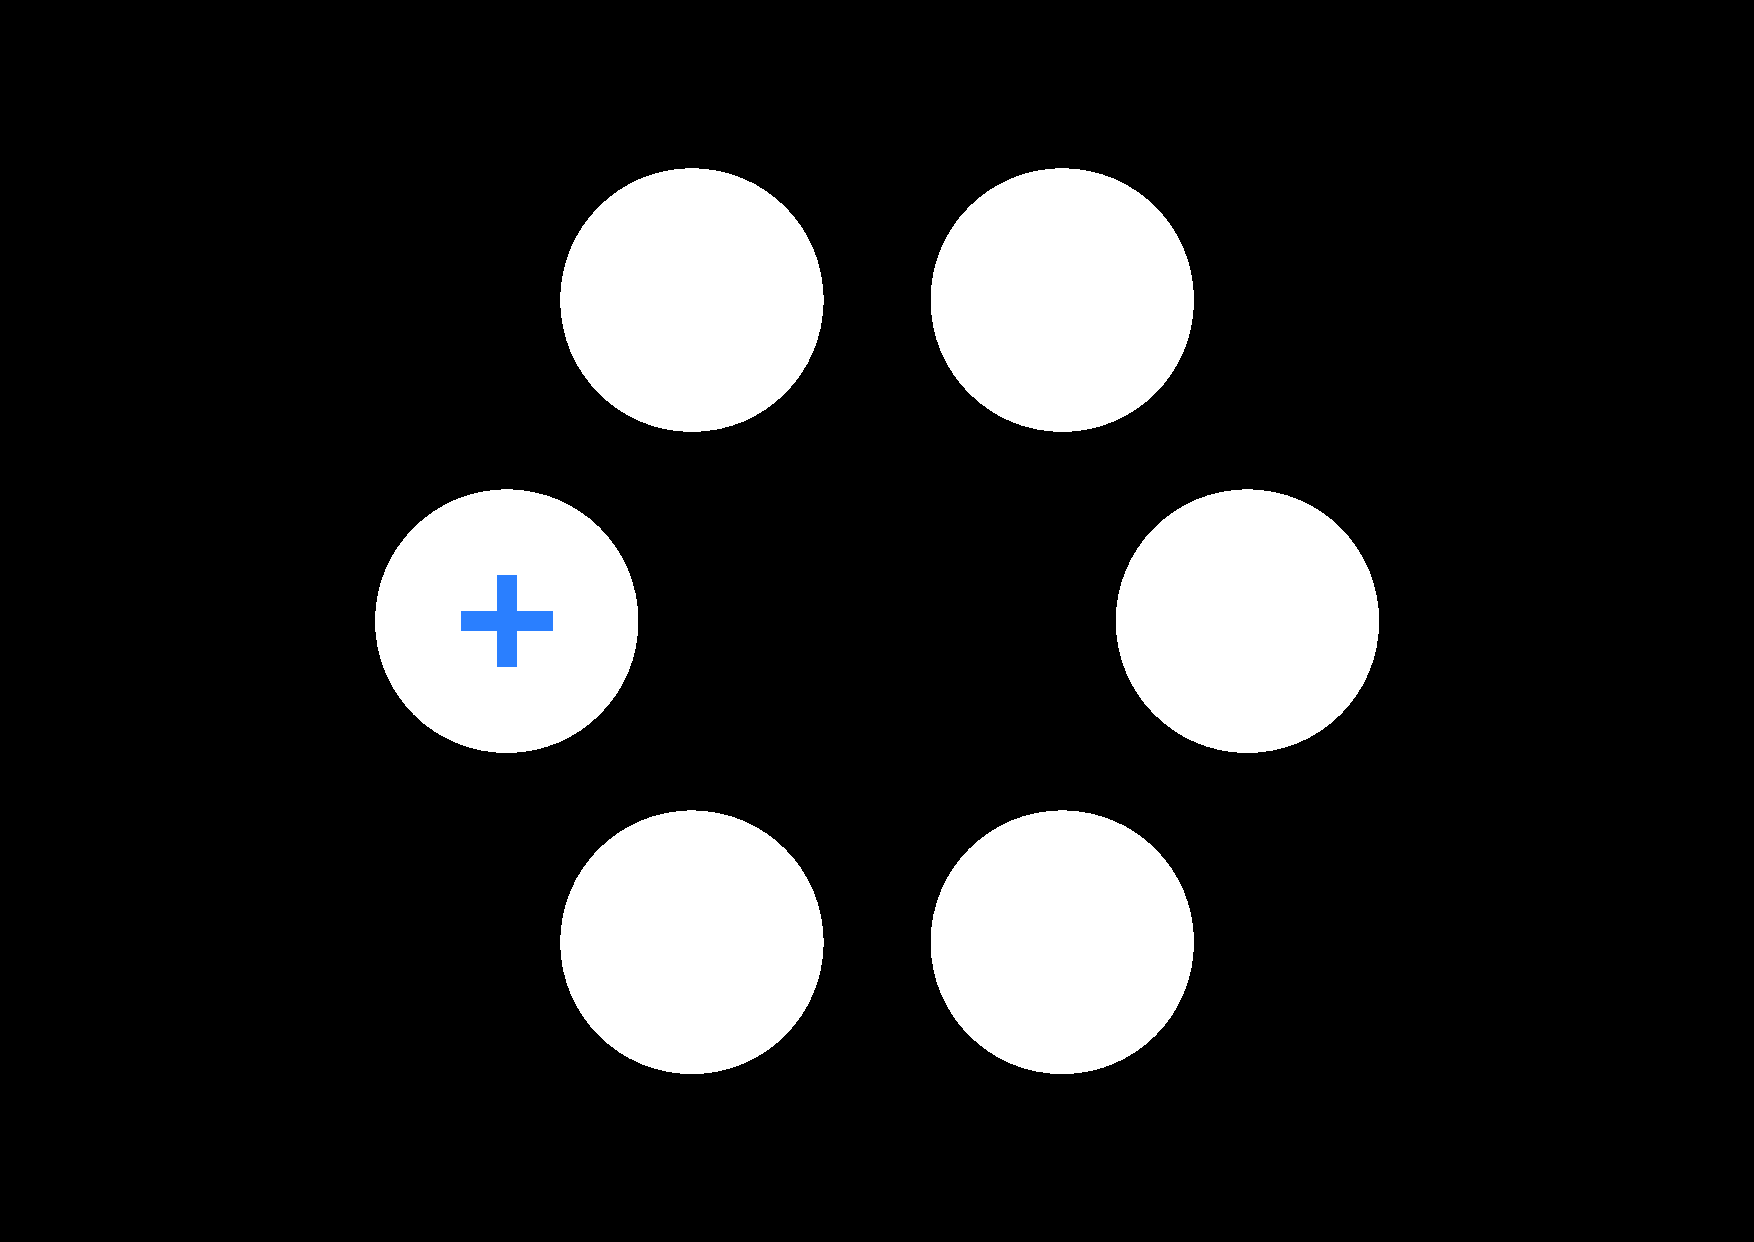
\includegraphics[width=\textwidth]{figures/stim_overt.pdf}
			\caption{Stimulation interface with 6 targets and fixation crosshair
				positioned for \emph{overt} \ac{vsa}.}
		\end{subfigure}\hfill%
		\begin{subfigure}[b]{.45\linewidth}
			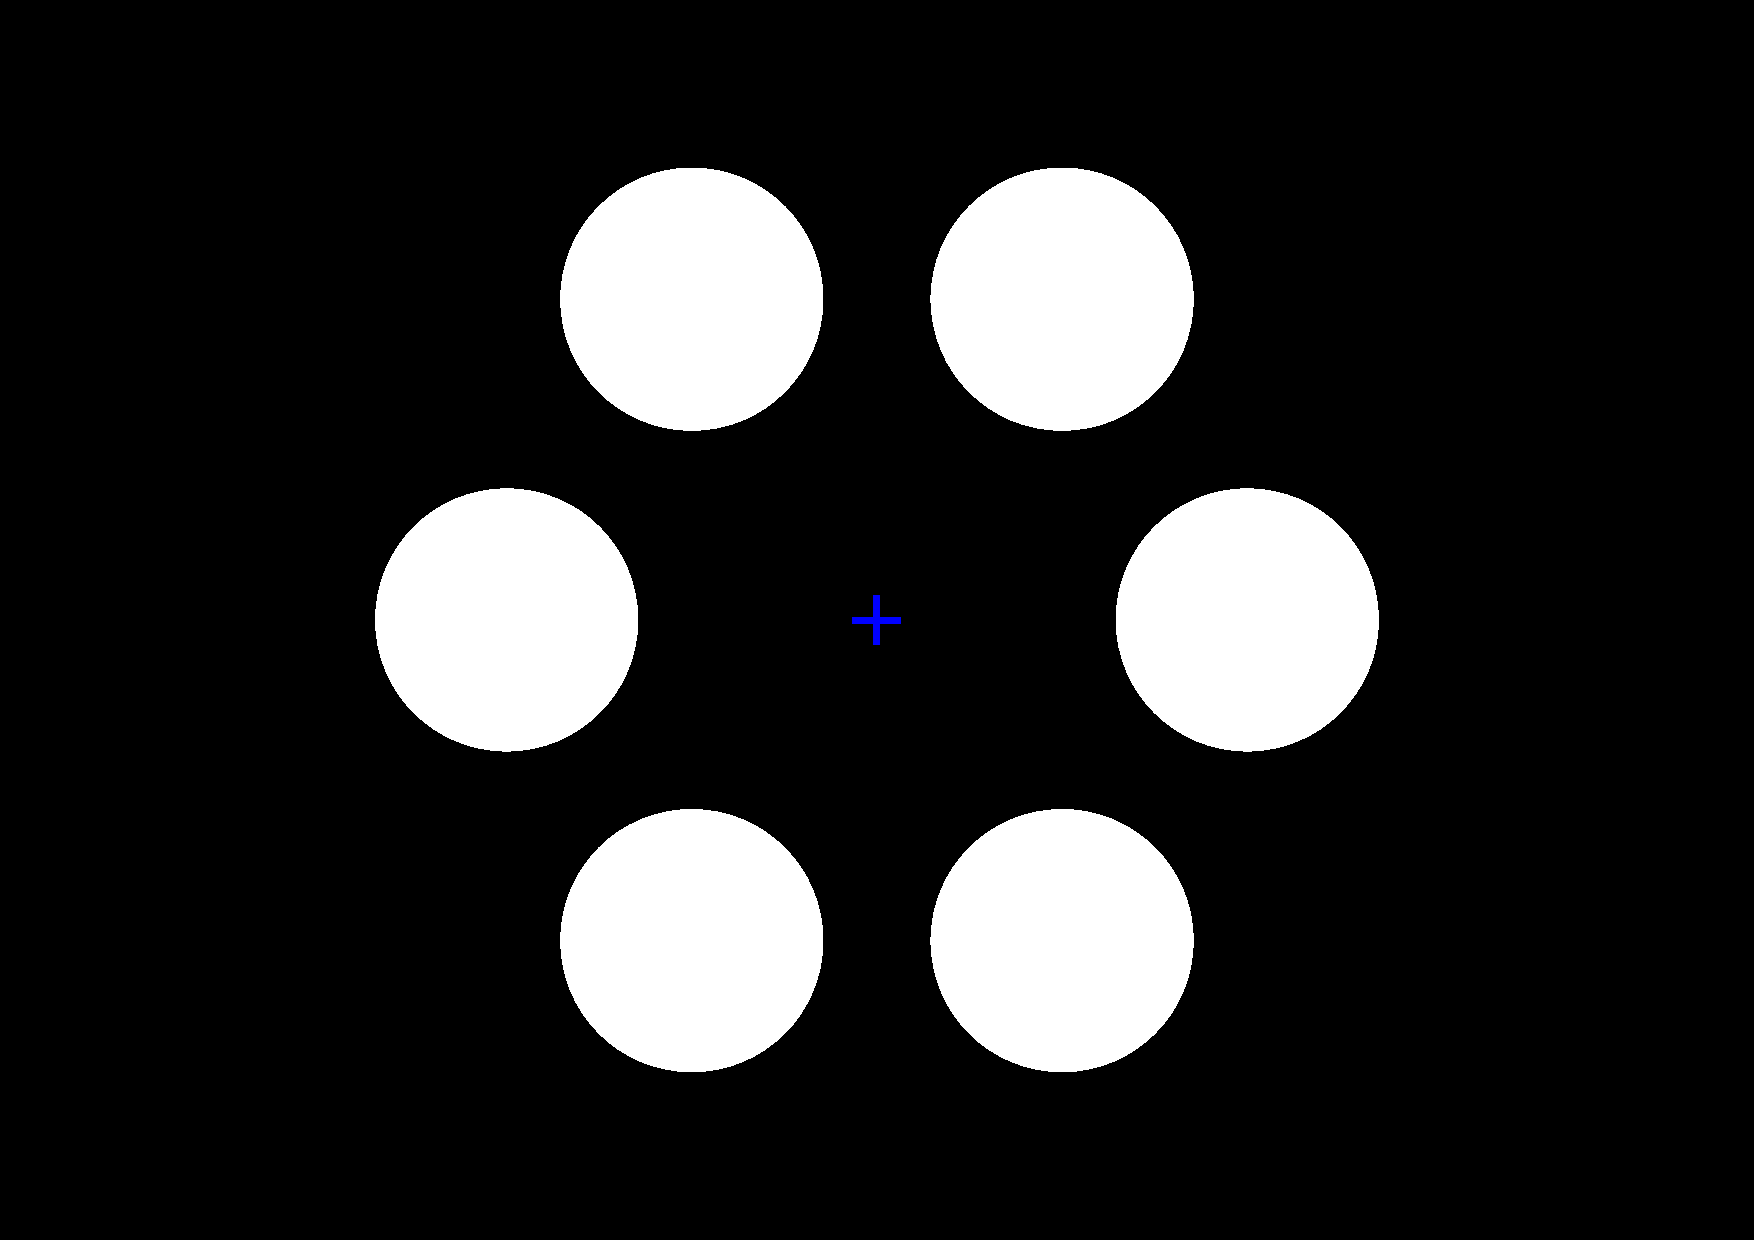
\includegraphics[width=\textwidth]{figures/stim_covert.pdf}
			\caption{In \emph{covert} \ac{vsa}, the fixation crosshair is placed in the
				center of the screen.}
		\end{subfigure}
		\smallskip

		\begin{subfigure}[b]{.45\linewidth}
			
\includegraphics[width=\textwidth]{figures/stim_free.pdf}
			\caption{In \emph{free} \ac{vsa}, no fixation crosshair is displayed.}
		\end{subfigure}\hfill%
		\begin{subfigure}[b]{.45\linewidth}
			
\includegraphics[width=\textwidth]{figures/stim_intense.pdf}
			\caption{Targets are intensified by enlarging them for 100 ms.}
		\end{subfigure}
	\end{minipage}

	\caption{%
		Stimulation and recording setup for the oddball \ac{bci} experiment
		with different \ac{vsa} conditions
	}%
	\label{fig:methods/stimulation/stimulation}
\end{figure*}

Three different \ac{vsa} settings were explored.
In the overt \ac{vsa} setting, the participant was instructed to fixate on the cued target or
to try this to the maximum extent of their visual skill, even if experiencing
slight discomfort.
In the covert \ac{vsa} setting, the participant was instructed to fixate on the center of the
screen, to the extent of their ability.
An additional \emph{free \ac{vsa}} setting was introduced.
Here, the participant was instructed to perform the task as they deemed most
comfortable.
This allowed us to investigate the user's natural way of operating the \ac{bci}
given their individual set of visual skills.
If the participant was not fully paralyzed, they were instructed not to move their head.
The cued \emph{split attention} setting proposed
by~\textcite{VanDenKerchove2024} was not studied here, as we were interested
in natural \ac{vsa} operation settings for gaze-impaired individuals.

To make the interface suitable for use by individuals with
participants with neurological conditions~\cite{FriedOken2020}, the amount of blocks was reduced to 6 per \ac{vsa} setting.
In order to decrease task difficulty, \ac{isi} was increased to 200 with added random jitter uniformly distributed
between -50 ms and 50 ms.
The experiment also started with a training block in each condition, where the
participant was instructed with oral feedback on their counting accuracy to ensure they
understood and were able to perform the task.


\subsection{\Ac{eeg} data collection \& preprocessing}

During the recording session, participants were positioned in their wheelchair in front of a table.
Stimuli were presented on an Acer Predator Helios laptop with an 18" screen (Acer,
Inc., Taiwan) placed at a 60 cm distance.
A Cedrus StimTracker (Cedrus Corp., CA, USA) ensured synchronization of stimuli with the
recorded \ac{eeg}.

\Ac{eeg} was recorded at 1000 Hz using the Neuroscan Neuvo portable amplifier (Compumedics Neuroscan,
Australia) connected to a second laptop for registration.
The \ac{eeg} headset used 18 active AgCl electrodes (EASYCAP GmbH, Germany) placed on a cap
according to the international 10-20 layout.
Using electrolyte gel, electrode impedances were reduced below 10 k$\Omega$.
Additionally, the \ac{eog} was recorded.

The \ac{eeg} was band-pass filtered between 0.5 and 16 Hz.
Bad channels were rejected using the RANSAC algorithm~\cite{Fischler1981}
and visual inspection.
Next, the \ac{eeg} was re-referenced to the average of mastoid electrodes TP9
and TP10, and \ac{ica} was performed to reject artifactual components based on
correlation with the \ac{eog} or by visual inspection.
Epochs were cut from -0.1 to 0.9 s relative to stimulus onset, and no baseline
correction was performed.

\subsection{\Acs{bci} decoding}

We evaluated the recorded \ac{eeg} data using the \ac{wcble}~\cite{VanDenKerchove2024}
and \ac{tlda}~\cite{Sosulski2022}
classifiers, as well as the Riemannian approach XDAWNCov+TS+LDA~\cite{Cecotti2017}.
For \ac{wcble}, a region of interest from 0 ms to 800 ms relative to stimulus
onset was used while the epoch was cropped to -100 ms to 900 ms. For the other
decoders, the epoch was cropped between 0 ms and 800 ms, which resulted in maximal
accuracy.
Decoding scores were obtained using 6-fold cross-validation where folds corresponded to
stimulation blocks.

\section{Results}



\subsection{Eye tracking analysis}%
\label{sec:patients/outcomes/gaze}
Given their eye motor impairment as listed in~\cref{tab:patients/eye}, we aimed to clarify the
capabilities of the participants in performing overt \ac{vsa} and central gaze fixation and to
assess the relevance of these settings when gaze is not cued.
\Cref{fig:patients/gaze} maps gaze position relative to the targets
across conditions.
These results should be interpreted with care, as the eye tracker partially
relies on intact eye motility.
The participant's position relative to the eye tracker might have shifted
throughout the experimental session despite our best efforts, due to e.g.\ a
regular need for aspiration of the tracheostoma of some participants
\begin{figure*}
	\resizebox{\linewidth}{!}{%
		\import{figures}{fig_gaze.pgf}%
	}%
	\caption{%
		Distribution of the recorded gaze position during the experimental session in the three \ac{vsa}
		conditions.
		Crosshairs represent stimulus positions, with positions cued during
		the given condition indicated in red.
		Subjects PB2 and PC4 preferred covert \ac{bci} operation, with PB2 resting gaze
		near the middle of the screen, and PC4 near the bottom.
		A high-resolution, non-downsampled figure is available as Additional file 1.
	}%
	\label{fig:patients/gaze}
\end{figure*}

PA1 had relatively intact gaze control and was able to correctly perform the
cued overt and covert settings.
When gaze was uncued, he fixated on the cued target.
This was also mostly the case for PB1, although eye tracking revealed that he
chose not to perform central gaze fixation when cued in at least one of the
stimulation blocks. We were unable to record his gaze near the bottom-left
stimulus position, either due to eye tracker failure or because the participant
was not comfortable fixating on this position.
Eye tracker calibration did not succeed for subject PB4, but given the
transformation of gaze positions to the stimulus space, they were assumed to
be overtly performing the free task.

PB2 was able to perform overt \ac{vsa} and central fixation to some extent,
yet eye tracking shows a larger spread in gaze position compared to
PA1 and PB1.
In the free \ac{vsa} condition, however, she preferred to attend
stimuli covertly when the gaze was uncued.
This was confirmed by the participant.

The overt and central gaze fixation settings were also not properly adapted to
participant PC4.
In the free \ac{vsa} condition, eye tracker results show that his gaze was usually near the
bottom two targets, indicating some degree of covert or split \ac{vsa}.

Technical difficulties were encountered while recording gaze position with the
Tobii X2-30
Compact for participants PC2 and PC3, since they both had one eye that was
occluded respectively by the prism glass and the eyelid.
Both participants reported they could not fixate on some of the
stimuli.

\subsection{\Acs{bci} decoding performance}

\Cref{fig:patients/decode} shows cross-validated single-trial target selection
accuracy for the evaluated \ac{vsa} settings for the different decoders.
A full table of results is available as Additional file 2.
Accuracy results do not reveal a clear trend in decoder performance per
condition.
In the covert \ac{vsa} setting with cued central gaze fixation, accuracy
deteriorated overall.
Target selection accuracy this task was around chance level ($\frac{1}{6}$) for
participants PB4, PC2 and PC3.

\Ac{wcble} did not improve over the accuracy of \ac{tlda} in the free \ac{vsa} setting, but
XDAWNCov+TS+LDA accuracy was slightly lower here, though not
significantly.
More interestingly, we noticed that accuracies of the decoders in free
\ac{vsa} were close to those in the overt \ac{vsa}.
A substantial decrease in accuraciy from the overt setting to the free
setting was observed for subjects PC2, PC3 and PC4 who had the most severe eye
motor impairment.
For PB2, who relied on covert \ac{vsa} during the uncued free \ac{vsa}
according to gaze tracking setting, the decrease in accuracywas also
present.
\begin{figure*}
	\sffamily
\begin{tikzpicture}[trim axis group left]

  \begin{groupplot}[
    group style={%
      group size=3 by 1,
      horizontal sep=10pt,
      ylabels at=edge left,
      yticklabels at=edge left,
    },
    ybar,
    ymin=0, ymax=105,
    ytick={0,20,40,60,80,100},
    xtick={0,1,2,3,4,5,6},
    xticklabels={PA1,PB1,PB2,PB4,PC2,PC3,PC4},
    xtick pos=bottom,
    ymajorgrids=true,
    xlabel={subject},
    ylabel={target selection accuracy (\%)},
    width=0.33\linewidth-5pt,
    scale only axis,
    /pgf/bar width=0.008\linewidth,
    cycle list/Set2-3,
    every axis plot/.append style={fill},
    every axis plot post/.append style={error bars/.cd, error bar style={color=gray}},
  ]

    \newcommand{\drawBarPlot}[2]{%
  	  \pgfplotstableread[col sep=comma]{data/decode_results_#1_#2_viz.csv}\datatable
  	  \addplot+[error bars/.cd, y dir=both, y explicit]
        table[
          x=subject_index,
          y=test_single_trial_accuracy-mean,
          y error minus=test_single_trial_accuracy-ci_minus,
          y error plus=test_single_trial_accuracy-ci_plus,
          col sep=comma
        ] {\datatable};
      }

    \newcommand{\drawRepMarker}[5]{%
  	  \pgfplotstableread[col sep=comma]{data/decode_results_#1_#2_viz.csv}\datatable
      \addplot+[only marks, mark=#5, mark size=2pt]
        table[
          x expr=\thisrow{subject_index} + #4,
          y=test_accuracy_reps_#3-mean,
          col sep=comma
        ] {\datatable};

    }

    \newcommand{\drawChanceLevel}{%
	    \draw[gray, dashed] (axis cs:-1,16.66666667) -- (axis cs:7,16.66666667);
    }

    \newcommand{\offset}{0.3}

    %% Plot overt
    \nextgroupplot[title=Overt \ac{vsa}]
    % Draw repetition performance
    \drawRepMarker{overt}{WCBLE}{5}{-\offset}{diamond}
    \drawRepMarker{overt}{tLDA}{5}{0}{diamond}
    \drawRepMarker{overt}{XDAWNCov+TS+LDA}{5}{\offset}{diamond}
    \drawRepMarker{overt}{WCBLE}{10}{-\offset}{square}
    \drawRepMarker{overt}{tLDA}{10}{0}{square}
    \drawRepMarker{overt}{XDAWNCov+TS+LDA}{10}{\offset}{square}
	  % Bar plot
    \drawBarPlot{overt}{WCBLE}
    \drawBarPlot{overt}{tLDA}
    \drawBarPlot{overt}{XDAWNCov+TS+LDA}
    % Draw chance level
    \drawChanceLevel

    %% Plot overt
    \nextgroupplot[title=Covert \ac{vsa}]
	  % Bar plot
    \addlegendimage{empty legend};
    \addlegendentry{\textbf{Decoder}};
    \drawBarPlot{covert}{WCBLE}
  	\addlegendentry{WCBLE};
    \drawBarPlot{covert}{tLDA}
  	\addlegendentry{tLDA};
    \drawBarPlot{covert}{XDAWNCov+TS+LDA}
  	\addlegendentry{XDAWNCov+TS+LDA};
    % Draw repetition performance
    \drawRepMarker{covert}{WCBLE}{5}{-\offset}{diamond}
    \drawRepMarker{covert}{tLDA}{5}{0}{diamond}
    \drawRepMarker{covert}{XDAWNCov+TS+LDA}{5}{\offset}{diamond}
    \drawRepMarker{covert}{WCBLE}{10}{-\offset}{square}
    \drawRepMarker{covert}{tLDA}{10}{0}{square}
    \drawRepMarker{covert}{XDAWNCov+TS+LDA}{10}{\offset}{square}
    %% Draw chance level
    \drawChanceLevel

    %% Plot overt
    \nextgroupplot[title=Free \ac{vsa}]
    % Draw repetition performance
    \drawRepMarker{free}{WCBLE}{5}{-\offset}{diamond}
    \drawRepMarker{free}{tLDA}{5}{0}{diamond}
    \drawRepMarker{free}{XDAWNCov+TS+LDA}{5}{\offset}{diamond}
    \drawRepMarker{free}{WCBLE}{10}{-\offset}{square}
    \drawRepMarker{free}{tLDA}{10}{0}{square}
    \drawRepMarker{free}{XDAWNCov+TS+LDA}{10}{\offset}{square}

	  % Bar plot
    \drawBarPlot{free}{WCBLE}
    \drawBarPlot{free}{tLDA}
    \drawBarPlot{free}{XDAWNCov+TS+LDA}
    %% Draw chance level
    \drawChanceLevel

  \end{groupplot}
\end{tikzpicture}%

	\caption{%
		Decoding performance in different \ac{vsa} settings reported as
		single-trial target selection accuracy (\%).
		Accuracy in free \ac{vsa} is generally on par with the overt \ac{vsa}
		setting.
		In the covert \ac{vsa} setting with central gaze fixation, accuracy is lower, but can
		be improved with the \ac{wcble} decoder.
		Whiskers indicate 95\% confidence intervals determined using 10,000 bootstrapping
		repetitions. Dashed line indicates the chance level accuracy. Diamond
		markers indicate target selection accuracy using the median score for five stimulation
		repetitions. Square markers indicate target selection accuracy for 10
		stimulation repetitions.
		($\frac{1}{6}$).
	}%
	\label{fig:patients/decode}
\end{figure*}

\subsection{Cross-condition decoder training and evaluation}%
\label{sec:patients/outcomes/cross}

As an alternative approach to selecting the most suitable decoder, we used
\ac{tlda} as the base decoder and verified whether accuracy could be improved
if \ac{bci} users with gaze impairment performed the decoder training session
session relying maximally on their residual gaze control.
A full table of results is available as Additional file 3.

\Cref{fig:patients/cross} shows that for participants PB1 and PC2 covert \ac{vsa} decoding
improved when training with overt \ac{vsa}.
Note that, according to eye tracking data, participant PB1, PB4, and PC4 did not
always perform cued central gaze fixation in the covert \ac{vsa} setting,
which might have affected the results.
\begin{figure*}
	\sffamily
\begin{tikzpicture}[trim axis group left]

  \begin{groupplot}[
    group style={%
      group size=3 by 1,
      horizontal sep=10pt,
      ylabels at=edge left,
      yticklabels at=edge left,
    },
    ybar,
    ymin=0, ymax=100,
    ytick={0,20,40,60,80,100},
    xtick={0,1,2,3,4,5,6},
    xticklabels={PA1,PB1,PB2,PB4,PC2,PC3,PC4},
    xtick pos=bottom,
    ymajorgrids=true,
    xlabel={subject},
    ylabel={target selection accuracy (\%)},
    width=0.33\linewidth-5pt,
    scale only axis,
    /pgf/bar width=0.008\linewidth,
    cycle list/Set2-3,
    every axis plot/.append style={fill},
    every axis plot post/.append style={error bars/.cd, error bar style={color=gray}},
  ]

    \newcommand{\drawBarPlot}[2]{%
  	  \pgfplotstableread[col sep=comma]{data/cross_results_#1_#2_viz.csv}\datatable
  	  \addplot+[error bars/.cd, y dir=both, y explicit]
        table[
          x=subject_index,
          y=test_single_trial_accuracy-mean,
          y error minus=test_single_trial_accuracy-ci_minus,
          y error plus=test_single_trial_accuracy-ci_plus,
          col sep=comma
        ] {\datatable};
      }

    \newcommand{\drawChanceLevel}{%
	    \draw[gray, dashed] (axis cs:-1,16.66666667) -- (axis cs:7,16.66666667);
    }


    %% Plot overt
    \nextgroupplot[title=Overt \ac{vsa} evaluation]
	  % Bar plot
    \drawBarPlot{overt}{overt}
    \drawBarPlot{covert}{overt}
    \drawBarPlot{free}{overt}
    % Draw chance level
    \drawChanceLevel

    %% Plot overt

    \nextgroupplot[title=Covert \ac{vsa} evaluation]
	  % Bar plot
    \addlegendimage{empty legend};
    \addlegendentry{\textbf{Calibration setting}}

    \drawBarPlot{overt}{covert}
    \addlegendentry{overt \ac{vsa}};
    \drawBarPlot{covert}{covert}
    \addlegendentry{covert \ac{vsa}};
    \drawBarPlot{free}{covert}
    \addlegendentry{free \ac{vsa}};
    %% Draw chance level
    \drawChanceLevel

    %% Plot overt
    \nextgroupplot[title=Free \ac{vsa} evaluation]
    % Draw repetition performance
	  % Bar plot
    \drawBarPlot{overt}{free}
    \drawBarPlot{covert}{free}
    \drawBarPlot{free}{free}
    %% Draw chance level
    \drawChanceLevel

  \end{groupplot}
\end{tikzpicture}%

	\caption{%
		Decoding performance when calibrating the \ac{tlda} decoder in a given \ac{vsa}
		setting, and evaluating it in another, reported as
		single-trial \ac{rocauc}.
		Whiskers indicate 95\% confidence intervals determined using 10,000 bootstrapping
		repetitions.
		For participants PA1, PB2, and PC3, decoding accuracy in the covert \ac{vsa} setting with central gaze fixation
		improved when calibrating with overt gaze fixation.
	}%
	\label{fig:patients/cross}
\end{figure*}

\section{Discussion}

This study investigated the feasibility of a gaze-independent visual oddball
\acp{bci} for individuals with \ac{sspgi}.
While covert \ac{vsa} with cued, central gaze fixation resulted in reduced decoding
accuracy, likely due to increased task load, accuracy in free \ac{vsa} where gaze position is uncued can
yield performance comparable to explicitly cued overt \ac{vsa} for some
participants.
This suggests that the evaluated participants naturally integrate residual gaze control.
Training with cued, overt \ac{vsa} can improve accuracy in subsequent free \ac{vsa} conditions,
highlighting the potential benefits of leveraging this residual eye motor control
during the decoder training phase.
While gaze-independent BCIs show promise for individuals with \ac{sspgi},
usability and comfort remain critical considerations for real-world applications.
These results provide important insights into the optimization of visual BCIs for individuals with severe motor impairments and underscore the need for further research into adaptive decoding strategies and user-centered design.

\subsection{Gaze-independent operation \& decoding}
Due to the heterogeneous nature of the participants' conditions and the limited
number of participants, it is difficult to draw general conclusions.
This study should therefore be seen as a collection of case studies,
highlighting different obstacles encountered in developing gaze-independent
visual oddball \acp{bci} for individuals with \ac{sspgi}.
Nevertheless, we highlight some aspects that might be
of interest for the further development of this class of \acp{bci}.

True \emph{gaze-independent} visual \acp{bci} should not rely on gaze fixation.
Hence, our analysis centers around the free \ac{vsa} condition.
Eye tracking results presented in \cref{sec:patients/outcomes/gaze}
confirm our assumption that voluntary covert \ac{vsa} can
occur in individuals with \ac{sspgi}.
We also confirmed part of the results presented by \textcite{VanDenKerchove2024},
which state that decoding of covert \ac{vsa} with central gaze
fixation can be improved by accounting for latency jitter. We showed that this
also holds for some individuals with \ac{sspgi}, with PA1 and PC4 as examples.

Contrary to our assumptions, we have shown that accounting for latency jitter does not
necessarily improve covert \ac{vsa} when gaze fixation is not cued.
One possible explanation is that actively performing central gaze fixation
increases task load.
This, in turn, can reduce overall performance, even though the participant might
have otherwise performed covert \ac{vsa}, but would not be occupied with
maintaining strict central gaze fixation.
This extra task demand is not present in the free \ac{vsa} condition, so
there is less performance to be gained.
Furthermore, cued central gaze fixation combined with counting flashing stimuli
in the visual periphery is an explicit example of a dual task.
Dual tasks have been shown to increase P3 latency
jitter~\cite{Polich2007,Arico2014, VanDenKerchove2024},
which is what \ac{wcble} accounts for.
Hence, increased P3 jitter might be more related to maintaining central gaze fixation
than to the actual covert \ac{vsa} aspect.

The seemingly stable accuracy across overt and free \ac{vsa} could be
misinterpreted as an indication that the Hex-o-Spell \ac{bci} already works
well for individuals with \ac{sspgi}, and no optimization is
needed.
However, we assume that overt \ac{vsa} accuracy was also decreased in some
subjects or for some blocks if the participant was not able to comfortably
perform the task.
Nevertheless, the large difference between the free \ac{vsa} setting and the
covert \ac{vsa} setting
with central gaze fixation is food for thought about the applicability of
solutions developed with central fixation in mind.

Individuals with all except the most severe gaze impairments will likely retain
some capability to direct their gaze in visual \ac{bci} operation, which can
drastically boost accuracy.
Subject PB2 exemplifies this: his free \ac{vsa} decoding accuracy is above that in covert
\ac{vsa}, and eye tracking showed that he relied mostly
on overt \ac{vsa} when cued to do so, and mostly on covert \ac{vsa} when
gaze was uncued.
This is also supported by our results on cross-condition decoder training and evaluation presented
in \cref{sec:patients/outcomes/cross}, which show that leveraging residual
eye motor control to fixate targets during the decoder training phase can improve
decoding accuracy in some settings.
This is likely due to the increased P3 component amplitude in overt \ac{vsa},
which improves the discriminative power of a classifier trained on this data.
Cueing this overt gaze fixation only during the decoder training phase leaves the user
free to operate in the manner that is most comfortable in the
operation phase.
Early VEPs in the training data could also contribute in those cases where the participant was not
able to perform covert \ac{vsa} with central gaze fixation.

\subsection{Clinical implications}
The population of individuals with \ac{sspgi} is sparse, yet is regularly
confronted with major challenges.
As opposed to individuals in a vegetative or severe minimally conscious state,
they demonstrably have the intent and capability to communicate their thoughts
and desires to their clinicians, caregivers and social network.
These capabilities, however, are severely limited by their condition,
reducing the effectiveness and efficiency of communication.
Hence, finding a way to fill in this gap is a major issue in the care of
individuals with \ac{sspgi}.

Our work shows that some patients might benefit from visual \acp{bci}
for home use or in the clinical setting.
While the proposed communication protocol is a proof of concept with a limited degree
of freedom, it is a step towards applications like textual communication and
environment or home automation control that inherits the relatively high
information transfer rate of visual \acp{bci}.

Furthermore, our experiments revealed that the required technology and its
potential applications were generally well received by the participants and their
environment.
While the necessary visual attention task can be taxing if performed for
extended
periods of time, participants indicated that this was outweighed by the
potential to communicate in a more automated and autonomous way compared to
their current \ac{aac} solutions, which often required the help of a trained caregiver.

\subsection{Limitations \& recommendations}

Despite the insights gained on gaze-independent \ac{bci} approaches, certain limitations must be addressed in future research.
First and foremost, this study works with a limited sample size, which
does not represent the full spectrum of individuals with
\ac{sspgi} and their specific symptoms and skills.
Individuals with \ac{fa} met the inclusion criteria, but they are usually not
considered one of the typical interest groups for \ac{bci} communication assistive
technology, partly due to the rarity of the disease and partly due to its
progression.
It would be most interesting to verify these results with individuals with
\ac{lis} and no eye movement capability at all.

Another limiting factor is the difficulty experienced in correctly interpreting eye
tracker results in studies with individuals with gaze impairments.
If eye tracking is possible at all, it is not guaranteed that the user is able
to successfully perform the calibration procedure.
Further experiments should be carried out with a stationary eye tracker with
more advanced capabilities, although systems using a head fixator or headrest
should be avoided.
This is not practical when working with
wheelchair-bound individuals who might have undergone a tracheostomy and may
suffer from spasticity.
Given different more suited gaze tracking hardware, adapted to the participant's
conditions, analyses could be performed with a finer granularity by assessing
the gaze condition on a per-epoch basis.

To properly contextualize performance results, they should be coupled with
metrics evaluating the full scope of the user's requirements, with measures of
usability, comfort and perceived effort, like the NASA Task Load
Index~\cite{Hart2006}.
Decoding accuracy might, after all, be traded off for user comfort.
The perception of this type of \ac{bci} by the user might also be influenced by
performing the experiment in an on-line manner, providing immediate feedback
after selection and thus closing the loop.
In this study, user comfort in the different conditions was not objectively
measured.
Instead, it was assumed that participants operated most comfortably in the free
\ac{vsa} condition.
Even though participants reported that they could comfortably operate the
system, this must be confirmed with more quantitative assessments.
Eye motor disability could also have been assessed more quantitavely and
objectively~\cite{FriedOken2020}, using, e.g.,
the Revised Coma Recovery Scale~\cite{Giacino2004} or the NSUCO
oculomotor exam~\cite{Maples1992}, in order to relate them to the decoding or satisfaction results.

%Finally, the stimulation procedure parameters
%from~\textcite{VanDenKerchove2024} were adapted to make the counting task
%accessible to the \ac{bci} users with \ac{sspgi}.
%However, the number of repetitions and the \ac{isi} were not optimized to achieve
%maximal \ac{itr}.
%An interface that aims to maximize \ac{itr} could necessitate more or faster
%gaze redirections, which might result in different conclusions regarding the
%comfort and the impact of the retained visual skills.
%\todo{
%	conclusion: recommendation for more complete system integrating BCI and eye tracking, who could benefit. "Recommendation" in section header
%	select couple of patients with special needs and work with them for longer time, not necessary more patients to find significant results
%	here take some parts from thesis
%}

To optimize BCI user experience, research must extend beyond offline classification
performance and address the full scope of user interaction during online use.
Offline evaluation, while convenient, fails to capture critical factors such as
user engagement, learning effects, and true satisfaction.
A \ac{ucd} framework offers a structured approach to evaluate
effectiveness, efficiency, and satisfaction in realistic
settings~\cite{Standardization2009,Schreuder2013,Kuebler2014,Han2022}.
This includes transitioning from abstract stimuli to meaningful interfaces
providing immediate feedback, and evaluating performance metrics in real-time.
Satisfaction, a subjective yet vital component, should be assessed through
questionnaires after realistic online use~\cite{Kuebler2014}.
Decoder development, interface design, and paradigm selection should be
co-optimized, as improvements in decoding alone may be insufficient if the
paradigm does not align with the user’s abilities and preferences.
Ultimately, the goal is to design a usable system for individuals with
specific impairments, where longitudinal studies with targeted user groups or
individuals are required to evaluate system performance comprehensively.

Implementing such a user-centered approach requires early and active involvement
of individuals with SSPI throughout the research process~\cite{Standardization2009}.
Instead of a traditional bottom-up approach -- starting with healthy controls and
offline analysis -- similar future projects should begin directly with online experiments
in the target population, identifying challenges and iteratively optimizing the
system~\cite{FriedOken2020}.
This requires long-term collaboration with patient centers to ensure an involved
team of clinicians, occupational and speech therapists, and other caregivers, next to
further arrangements like ethical approval, and access to suitable infrastructure
from the onset.
Maintaining a functional in-house online \ac{bci}-\ac{aac} system facilitates iterative
development and realistic performance estimation, ensuring experimental settings
reflect practical use.
While this top-down approach may not suit novel \ac{bci} paradigms in early
development, it is appropriate for mature paradigms such as visual oddball
BCIs~\cite{Pan2022,Fouad2020}, where the main challenge lies in usability and
disseminating the technology to potential userssection

\acresetall%
\section{Conclusion}
This study explored the usability of \ac{eeg}-based gaze-independent visual BCIs in
individuals with \ac{sspgi}, focusing on the impact of eye motor impairments
on performance.
Our results demonstrate that a visual \ac{bci} gaze-independent operation is feasible
for some of these individuals.
They might either achieve sufficient decoding accuracy despite their eye
motor impairment, or performance can be enhanced by careful, individual
adaptation the decoding strategies.
The free \ac{vsa} condition yielded decoding accuracy comparable to overt \ac{vsa} in some participants, suggesting that users may naturally integrate residual gaze control.
Additionally, training under overt \ac{vsa} conditions improved accuracy in
subsequent covert or free \ac{vsa} operation, highlighting the potential benefits of
leveraging residual eye motor capabilities during decoder training.

While these findings are promising, future work should include larger
participant groups, refine stimulation paradigms, and incorporate
user-centered assessments of comfort and usability to actively develop usable
solutions.
Ultimately, optimizing gaze-independent BCI designs could enhance communication
options for individuals with severe motor and speech impairments, particularly
those who struggle with conventional eye-tracking technologies.

\printacronyms%

\section*{Declarations}
\subsection*{Ethics approval and consent to participate}
Ethical approval for this multi-center study was obtained from the Ethics
Commission of the University Hospitals Leuven (S62547),
and prior informed consent to participate  was obtained from
all participants included in this study.

\subsection*{Consent for publication}
Prior informed consent for publication of the reported data was obtained from
all participants included in this study.

\subsection*{Availability of data and materials}

The datasets generated and/or analysed during the current study are not publicly
available due to the policies in agreement with the ethical approval to protect
sensitive personal information, but are available from the corresponding author
on reasonable request.

\subsection*{Competing interests}
The authors declare no competing interests.

\subsection*{Funding}
AVDK is jointly funded by the special research fund of the KU Leuven (GPUDL/20/031) and
the University of Lille under the Global PhD Scholarship Programme, and by
the Belgian Fund for Scientific Research – Flanders (G0A4321N).
MMVH is supported by research grants received from the European Union’s
Horizon Europe Marie Sklodowska-Curie Action program
(grant agreement No. 101118964), the European Union’s Horizon 2020 research and
innovation program (grant agreement No. 857375), the special research fund of
the KU Leuven (C24/18/098), the Belgian Fund for Scientific Research – Flanders
(G0A4118N, G0A4321N, G0C1522N), and the Hercules Foundation (AKUL 043).
HSM and FC are supported by the RITMEA project co-financed by the
European Regional Development Fund of the European Union, the French state,
and the Hauts-de-France Region Council.
\todo{%
	If you are an academic partner and received governmental or project
	funding during the project please let me know in order to complete this
	section.
}

\subsection*{Author's contributions}
AVDK conceptualized the work and performed the analyses
presented this study, under supervision of HSM, FC and MMVH.
JM assisted in data collection, conceptualization and data analysis.
AW and MDM provided paramedical support in participant recruitment,
care and communication.
DG assisted in participant recruitment at the Univesity Hospitals Leuven NMRC under clinical supervision of PVD.
ES supervised participant recruitment at TRAINM.
EA provided clinical supervision during conceptualization, experimentation, supervised recruiting at Fondation Partage et Vie and contributed the neuro-ophthalmologic diagnoses.
Al authors read and approved the final manuscript.


\subsection*{Acknowledgements}
We acknowledge the active support of clinical, paramedical, management and
administration staff at the UZ Leuven Neuromuscular Reference Center
TRAINM Neuro Rehab Clinics Antwerp and the Fondation Partage et Vie Loos.
We would also like to thank the other colleagues at the KU Leuven Computational
Neurosciences research group and the University of Lille BCI team
for their general support.

\section*{Additional files}

\begin{enumerate}
	\item \textbf{Additional file 1} \\
	      \emph{Format}: portable network graphics file (.png) \\
	      \emph{Title}: Heatmap of gaze location per VSA condition.\\
	      \emph{Description}: High-resolution heatmap of the distribution of recorded
	      gaze position during the experimental session in the three VSA
	      conditions.
	      Crosshairs represent stimulus positions, with positions
	      cued during the given condition indicated in red.
	\item \textbf{Additional file 2} \\
	      \emph{Format}: comma-separated values file (.csv) \\
	      \emph{Title}: Decoding performance per patient.
	      \emph{Description}: Full table of decoding target selection accuracies
	      per patient, decoder and VSA condition.
	\item \textbf{Additional file 3} \\
	      \emph{Format}: comma-separated values file (.csv) \\
	      \emph{Title}: Cross-condition decoding performance per patient.
	      \emph{Description}: Full table of cross-validated, cross-condition
	      decoding target selection accuracies per patient and decoder.
\end{enumerate}


\printbibliography%


\appendix
\section{Clinical evaluation of participants}
\label{app:clinical-eval}

\paragraph{PA1}
\emph{Diagnosis:} 58 y.o., originally left-handed male diagnosed with bulbar-onset
\ac{als} 2 years prior at age 56.
Recently, symptoms started progressing more on the right side.
and resulted in immobility of the left limbs and partial immobility of the right
limbs, but right arm and finger movement were possible, albeit with effort.
\emph{Presentation:} PA1 presented lying reclined in a hospital bed, the
experimental setup was positioned on a movable folding table.
\emph{Communication:} Due to complete anarthria, PA1 communicated using vocal
grunts and a text-to-speech
\ac{aac} tablet operated with the right hand.
\emph{Eye movements:} He reported fatigue linked to his disease progression when
visually fixating for prolonged times, but otherwise reported no eye movement
abnormalities or visual defects.

\paragraph{PB1}
\emph{Diagnosis:} 41 y.o., originally left-handed male diagnosed with \ac{fa}
29 years prior, at age 12.
Symptoms resulted in slowed, effortful body and limb movement and affected
fine motor control, and most severely affected the left side which made him
effectively right handed.
\emph{Presentation:} PB1 presented in an electric wheelchair, which was
positioned in front of a table with the experimental setup.
\emph{Communication:} Verbal communication was possible, but dysarthria resulted
in slowed, slurred speech.
He was able to effectively control a PC and a smartphone, but writing was difficult.
\emph{Eye movements:} PB1 reported impaired visual pursuit of moving targets and
fatigue and discomfort fixating.
Effectively, we noticed effort when making eye movements, which resulted in
large muscular artifacts registered in he \ac{eeg} and \ac{eog}
Additionally, he reported minor nystagmus which we also noticed in the horizontal
\ac{eog}.

\paragraph{PB2}
\emph{Diagnosis:} 43 y.o., right-handed female diagnosed with \ac{fa}
symptom-free at age 9, with symptom onset at age 12, 31 years prior to the
experiment.
Symptoms resulted in slowed, effortful body and limb movement and affected
fine motor control.
\emph{Communication:} Dysarthric, characterized by large effort necessary to speak.
Hand signaling was also often used, but also required effort.
\emph{Eye movements:} PB2 was affected by especially severe horizontal eye
oscillations with onset 10 years prior to the experiment.
Fixating was also fatiguing and uncomfortable, especially when not wearing
glasses.

\paragraph{PB4}
\emph{Diagnosis:} 48 y.o., right-handed male diagnosed with \ac{fa} 30 years
prior at age 18.
\emph{Presentation:} PB4 was not strictly wheelchair-bound.
\emph{Communication:} Speech was relatively fluent, only slightly slurred,
leading to mild dysarthria.
\emph{Eye movements:} Pursuit and fixation were impaired, as characterized by
self-reported fatigue and discomfort. Nystagmus.

\paragraph{PC2}
\emph{Diagnosis:} 43 y.o., originally right-handed male diagnosed with \ac{lis} due to
ischemic brain stem stroke 6 years prior, at age 37. He underwent a tracheostomy.
\emph{Presentation:} PC2 was seated in an electric wheelchair controlled by a
caregiver, and his head was fixated in a headrest.
This headrest contacted the \ac{eeg} cap occipitally and centrotemporally, which
interfered slightly with cap and electrode positioning and optimization.
Additionally, heavy movement artifacts were noticed in the \ac{eeg} due to the
combination of breathing, aspiration, the headrest and maintaining correct
positioning for the experiment.
The \ac{eeg} cap was held in place using a chest strap.
\emph{Communication:} PC2 was completely anarthric and had no preserved facial
movement. He communicated with caregivers by responding to prompted letters and
words with upwards eye movement signaling.
Additionally, he sometimes made use of an emergency button which he could
control with his left hand, the only extremity in which he had some residual
control capability.
\emph{Eye movements:}
Right eye: preserved vertical movement, paralysis of laterality to the right and to the left,
which resulted in the inability to perform horizontal movements.
Left eye: preserved vertical movement, adduction possible, abduction deficit.
Deviation in the left eye resulting in diplopia, corrected by a prism glass.
Self-reported tremors and fixation fatigue and discomfort.

\paragraph{PC3}
\emph{Diagnosis:} 43 y.o., right-handed female diagnosed with hemorrhagic stroke
4 years prior, at age 39. She was tetraplegic and underwent a tracheostomy.
\emph{Presentation:} PC3 was seated in an electric wheelchair
\emph{Communication:} PC3 was completely anarthric, but had sufficient residual
motor control to indicate letters and symbols on a letterboard by pointing with
movements of the right index finger and hand.
\emph{Eye moevements:}
Right eye: complete ptosis
When corrected, downward movement was preserved and incyclotorsion was possible
through preserved cranial nerve IV. Ophthalmoplegia in other directions.
Left eye: Limited of adduction, complete verticality, horizontal nystagmus.
Intermittend nystagmus.
Self reported involuntary saccades and fixation fatigue or discomfort.

\paragraph{PC4}
\emph{Diagnosis:} 54 y.o., originally right-handed male diagnosed with ischemic brainstem
stroke 11 years prior, at age 53. He is tetraplegic and underwent a tracheostomy.
Symptoms most pronounced on left side.
\emph{Presentation:} The tracheostomy resulted in frequent aspiration which
interfered with the experiment and recording.
This and other factors related to the condition and positioning in the wheelchair
resulted in large and frequent muscular and movement artifacts in the \ac{eeg}.
Head bobbing When concentrating on the experimental task.
\emph{Communication:} PC4 had sufficient residual motor control
to indicate letters and symbols on a letterboard by pointing with
movements of the right index finger and hand.
\emph{Eye movement:}
A corneal abcess in the left eye affected it's motility and resulted in deviation.
The left eye had poor vision (only able to
distinguish shapes) and could not be closed.
The right eye was not affected.
The deviation resulted in fatigue and discomfort fixating.
Hypermetropia.
\todo{this is self-reported, official oculomotor diagnosis needed}


%\setcounter{table}{0}
%\renewcommand{\thetable}{A\arabic{table}}


\end{document}
